\documentclass[aspectratio=169,t]{beamer}
\usepackage[utf8]{inputenc}
\usepackage[T1]{fontenc}
\usepackage[export]{adjustbox}
\usepackage{amssymb}
\usepackage{xcolor}


\title{CAMI2: Pathogen Detection}
\date{February, March 12th}
\author[PWD]{Prof. Dr.-Ing. Piotr Wojciech Dabrowski}
\titlegraphic{Bilder/logo.jpg}

\usepackage{HTWBeamerTemplate/beamerthemeHTW}
%\setbeameroption{show notes on second screen}

\subtitle{The case in a few slides}
\addbibresource{sources.bib}
\begin{document}

\setbeamertemplate{footline}[first]

\begin{frame}[noframenumbering]
    \titlepage
    \begin{textblock}{10}(4.75,15)
			\textcolor{white}{\cite{logo}}
    \end{textblock}
\end{frame}

\setbeamertemplate{footline}[presentationbody] 

\begin{frame}{Case description}
	\begin{itemize}
		\item 32 year old woman
		\item Vomiting, abdominal pain, strong nosebleeds
		\item ILI symptoms and diagnosis 4 and 5 days prior
		\item Returned from Turkey 9 days prior - no wildlife contact or raw meat consumption
	\end{itemize}
	\only<2->{Task: Send taxonomy IDs of pathogens found and taxonomy ID of causative agent based on NGS data from blood sample\\}
	\only<3->{Solution: Crimean-Congo hemorrhagic fever orthonairovirus (CCHFV)\\}
	\only<4->{...so why a virus for the first pathogen detection challenge?\\}
	\only<5->{...and what is special about real samples?}
\end{frame}

\begin{frame}{Is pathogen detection special?}
	\begin{tikzpicture}
		\node[inner sep=0pt] (hay) at (0,0)
			{
				\only<1-2>{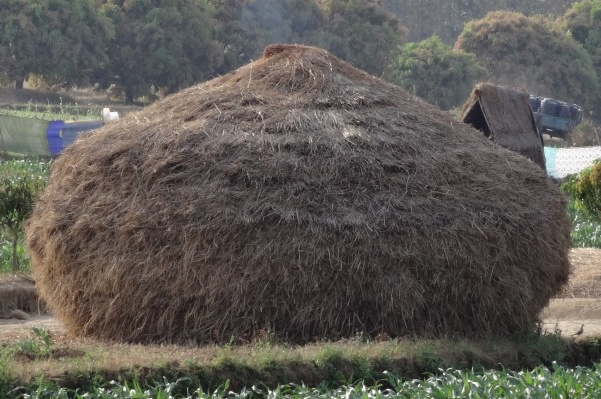
\includegraphics[width=6.5cm]{Bilder/haystack.jpg}} % https://pxhere.com/en/photo/993192
				\only<3->{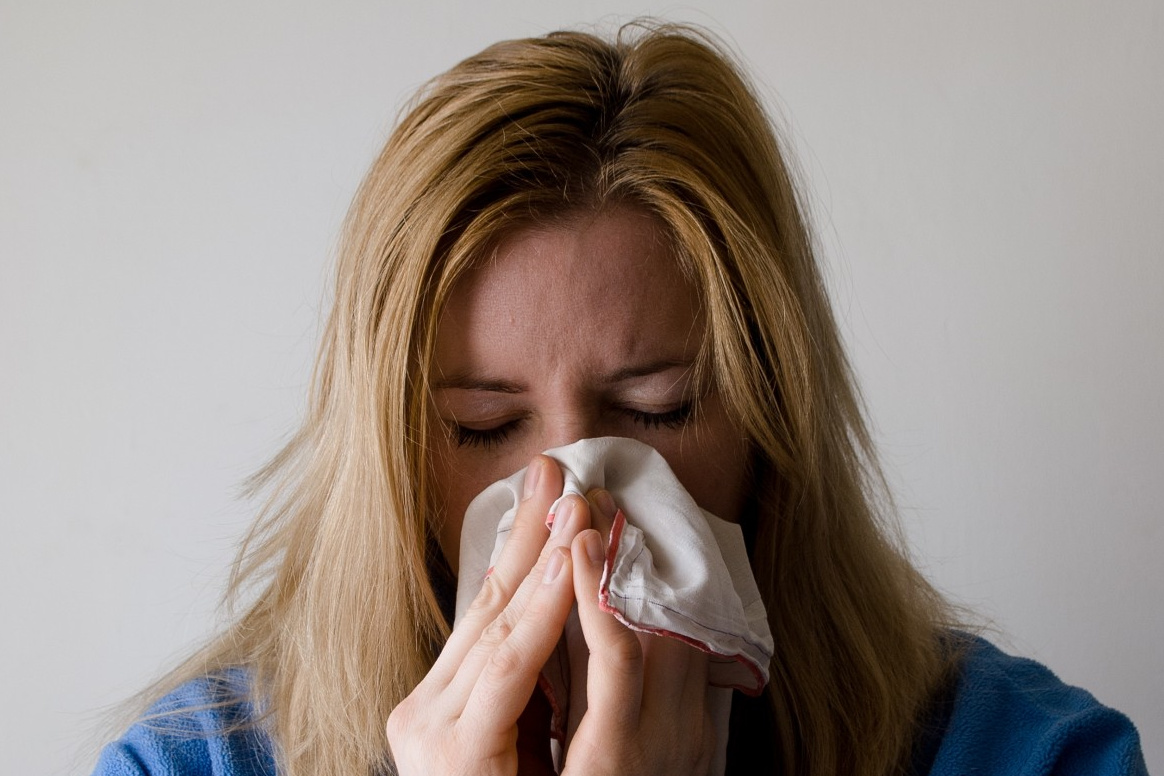
\includegraphics[width=6.5cm]{Bilder/patient.jpg}} % https://pxhere.com/en/photo/891702
			};
		\only<2->{
			\node[inner sep=0pt] (needles) at (7.5,0)
				{
					\only<2-3>{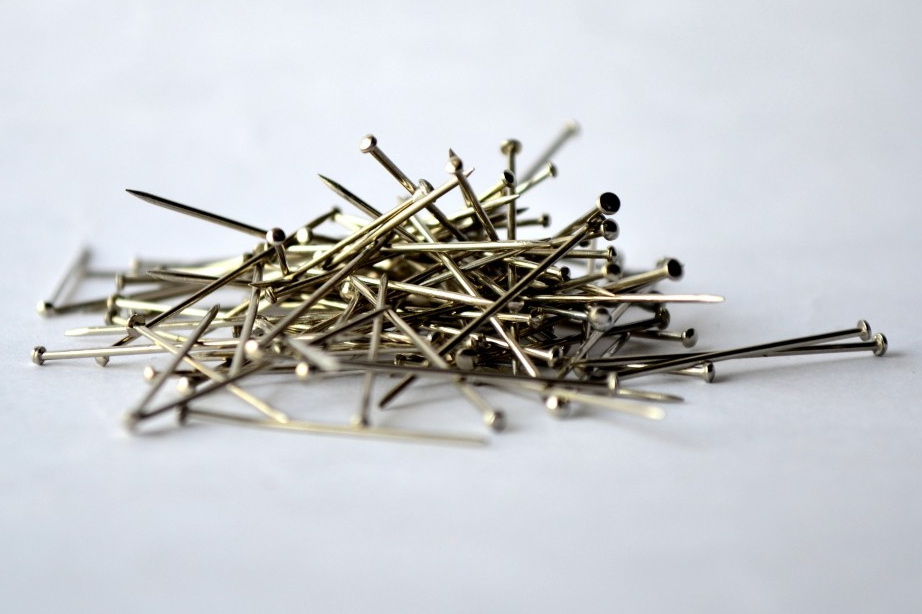
\includegraphics[width=6.5cm]{Bilder/needlestack.jpg}} % https://pxhere.com/en/photo/1349195
					\only<4->{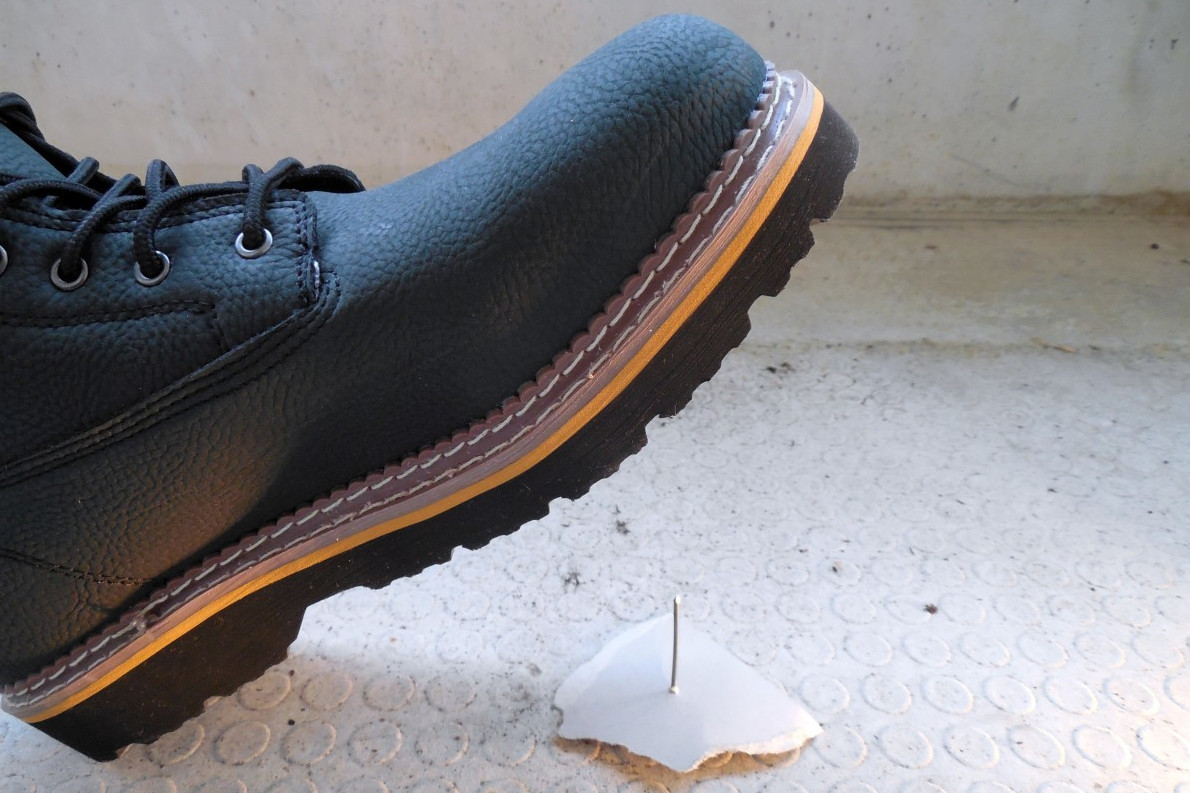
\includegraphics[width=6.5cm]{Bilder/needleshoe.jpg}} % https://pxhere.com/en/photo/682656
				};
			\draw[->,thick] (hay.east) -- (needles.west);
		}
		\only<1-2>{\draw node[xshift=-10, yshift=10] at (hay.south east) {\cite{hay}};}
		\only<3->{\draw node[xshift=-10, yshift=10] at (hay.south east) {\cite{patient}};}
		\only<2-3>{\draw node[xshift=-10, yshift=10] at (needles.south east) {\cite{needlestack}};}
		\only<4->{\draw node[xshift=-10, yshift=10] at (needles.south east) {\cite{accident}};}
	\end{tikzpicture}
\end{frame}

\begin{frame}{Are viruses easier?}
	\begin{tikzpicture}
		\node[inner sep=0] (vi) at (0,0)
			{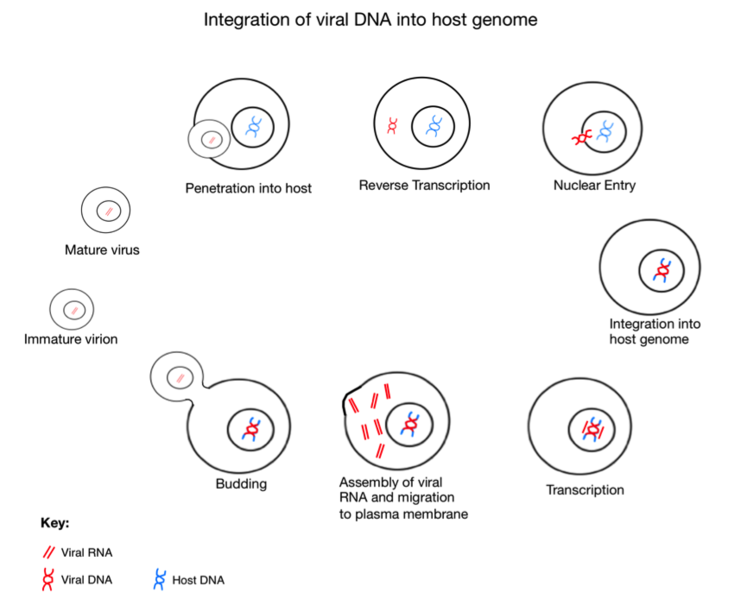
\includegraphics[width=0.53\textwidth]{Bilder/virusintegration.png}}; % 8% of human genome! https://commons.wikimedia.org/wiki/File:Integration_of_viral_DNA_into_host_genome.png
		\node[inner sep=0] (patho) at (8,0)
			{\only<2->{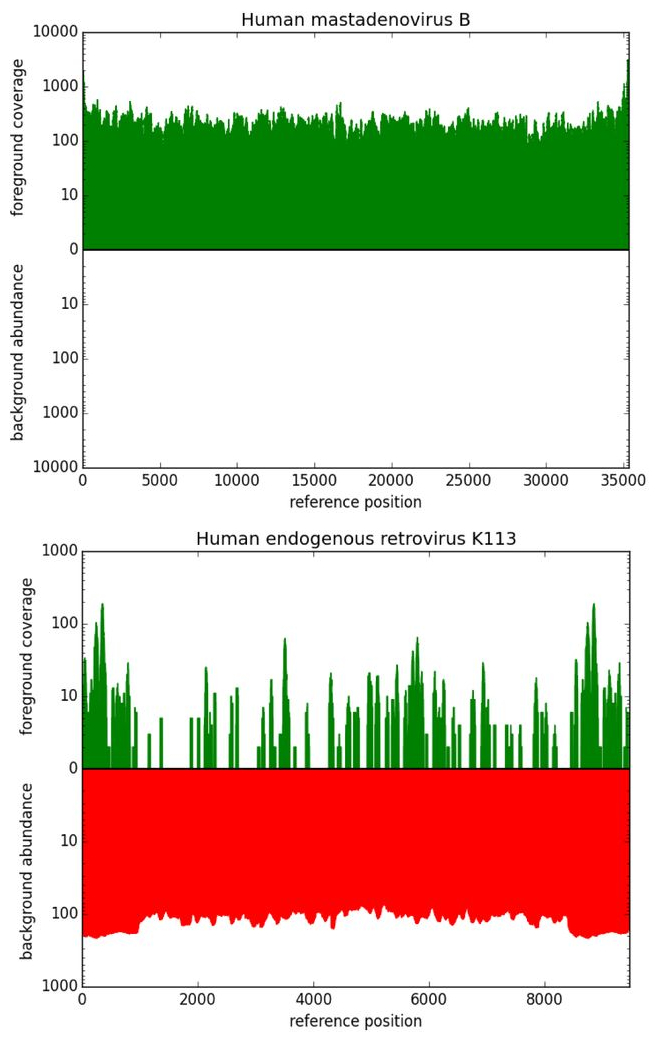
\includegraphics[width=0.26\textwidth]{Bilder/patholive.jpg}}}; % https://www.biorxiv.org/content/10.1101/402370v1 
		\draw node[xshift=-10, yshift=0] at (vi.south east) {\cite{virus}};
		\only<2->{\draw node[xshift=-10, yshift=0] at (patho.south east) {\cite{patholive}};}
	\end{tikzpicture}
\end{frame}

\begin{frame}{Privacy concerns}
	\begin{tikzpicture}
		\node[inner sep=0] (camels) at (0,0)
			{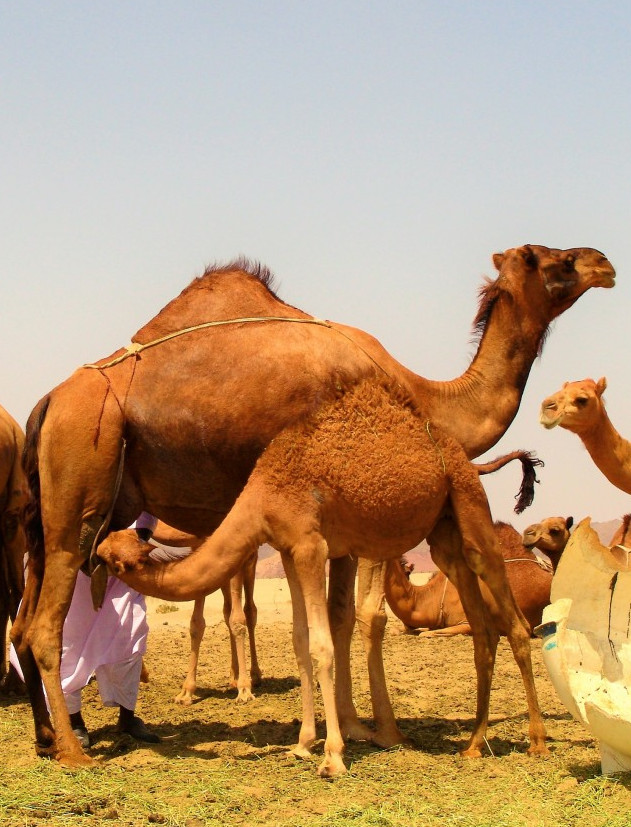
\includegraphics[height=0.7\textheight]{Bilder/camels.jpg}}; % https://pxhere.com/en/photo/1604201
		\node[inner sep=0] (face) at (5,0)
			{\only<2->{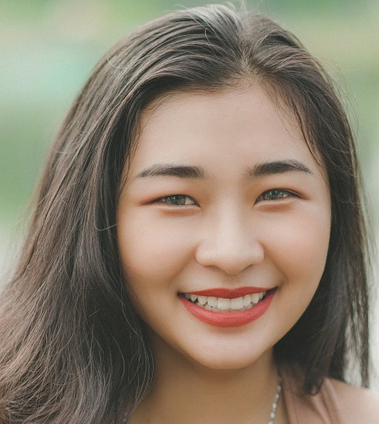
\includegraphics[width=0.3\textwidth]{Bilder/face.jpg}}}; % https://pxhere.com/en/photo/1419067
		\node[inner sep=0] (collage) at (10,0)
			{\only<3->{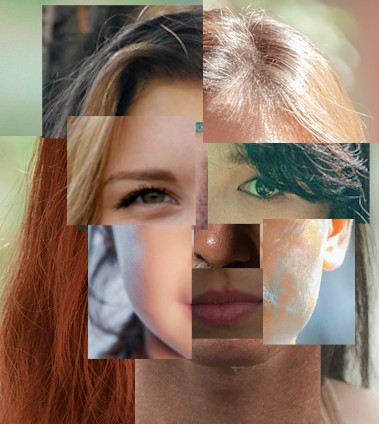
\includegraphics[width=0.3\textwidth]{Bilder/collage.jpg}}}; % https://pxhere.com/en/photo/1604201
		\only<3->{\draw[->,thick] (face.east) -- (collage.west);}
		\draw node[xshift=-10, yshift=10] at (camels.south east) {\cite{camels}};
		\only<2->{\draw node[xshift=-10, yshift=10] at (face.south east) {\cite{face}};}
	\end{tikzpicture}
\end{frame}

%\begin{frame}{Outline}
%	\begin{itemize}
%		\item Challenges in pathogen detection
%		\begin{itemize}
%			\item Why are bacteria hard?
%			\item Why viruses?
%		\end{itemize}
%		\item Challenges in clinical case preparation
%		\begin{itemize}
%		\end{itemize}
%	\end{itemize}
%\end{frame}

\begin{frame}[allowframebreaks]{Sources}
    \printbibliography
\end{frame}

\begin{frame}{Lizenz}
    \begin{center}
        
\includegraphics{Bilder/lizenz/by.png}\\
        Alle Inhalte außer dem HTW-Logo, für die keine Quelle angegeben ist, sind eigenes Material und unter CC-BY 4.0\\
        \url{https://creativecommons.org/licenses/by/4.0/}\\
        lizenziert.\\\vspace{0.5cm}
        Sämtliche Nutzungs- und Verwertungsrechte für das Logo der HTW Berlin in allen hier verwendeten Formen liegen ausschließlich bei der HTW Berlin:\\
        \url{https://corporatedesign.htw-berlin.de/logos/logo-htw-berlin/}
    \end{center}
\end{frame}



\end{document}
